% Created 2021-12-21 火 23:58
% Intended LaTeX compiler: pdflatex
\documentclass[lualatex,a4paper,12pt,report,ja=standard]{bxjsarticle}
\usepackage{bm}
\usepackage[sumlimits]{amsmath}
\usepackage{xcolor}
\usepackage{makeidx}
%\usepackage{newtxtext,newtxmath}
\usepackage{graphicx}
\usepackage[hidelinks,colorlinks=true,linkcolor=black]{hyperref}

%\usepackage[top=30truemm,bottom=30truemm,left=37truemm,right=18truemm]{geometry}
%%%%%% generate by 'org-latex-classes "luareport" %%%%%%


\author{osada-yum}
\usepackage{minted}
\date{\today}
\title{Org-babelの使用例}
\hypersetup{
 pdfauthor={mrt},
 pdftitle={Org-babelの使用例},
 pdfkeywords={},
 pdfsubject={},
 pdfcreator={Emacs 28.0.50 (Org mode 9.5)}, 
 pdflang={English}}
\begin{document}

\maketitle
\tableofcontents

\hypersetup{pdfauthor=osada-yum}

\section{Org-babelの設定}
\label{sec:orgae3fd0e}
\subsection{言語の設定}
\label{sec:orgfb068ed}
\texttt{C-c C-c} で実行.
\texttt{org-babel-do-load-languages} を使う.
\begin{minted}[frame=lines,framesep=2mm,linenos=true,baselinestretch=1.2,fontsize=\footnotesize,breaklines]{common-lisp}
(org-babel-do-load-languages
 'org-babel-load-languages
 '((emacs-lisp . t)
   (fortran    . t)
   (R          . t)))
(print org-babel-load-languages)
\end{minted}

\begin{verbatim}

((emacs-lisp . t) (fortran . t) (R . t))
\end{verbatim}

\subsection{言語の編集のときのmajor-modeの設定}
\label{sec:org869afa3}
\texttt{org-src-lang-modes} alistを追加する.
\begin{minted}[frame=lines,framesep=2mm,linenos=true,baselinestretch=1.2,fontsize=\footnotesize,breaklines]{common-lisp}
(add-to-list 'org-src-lang-modes '("fortran" . f90))
(print org-src-lang-modes)
\end{minted}

\begin{verbatim}

(("fortran" . f90) ("redis" . redis) ("php" . php) ("arduino" . arduino) ("C" . c) ("C++" . c++) ("asymptote" . asy) ("bash" . sh) ("beamer" . latex) ("calc" . fundamental) ("cpp" . c++) ("ditaa" . artist) ("dot" . fundamental) ("elisp" . emacs-lisp) ("ocaml" . tuareg) ("screen" . shell-script) ("shell" . sh) ("sqlite" . sql))
\end{verbatim}

\subsection{Fortran compilerの設定}
\label{sec:orgca107ae}
\texttt{org-babel-fortran-compiler} を変更する.
\begin{minted}[frame=lines,framesep=2mm,linenos=true,baselinestretch=1.2,fontsize=\footnotesize,breaklines]{common-lisp}
;; (setq org-babel-fortran-compiler "ifort")
;; (customize-set-value 'org-babel-fortran-compiler "ifort")
(print org-babel-fortran-compiler)
\end{minted}

\begin{verbatim}

"gfortran"
\end{verbatim}

\section{Fortran code block}
\label{sec:org052aee4}
\subsection{Fortran コードブロック}
\label{sec:org1587ae9}
\texttt{C-c C-c} で実行.
\begin{minted}[frame=lines,framesep=2mm,linenos=true,baselinestretch=1.2,fontsize=\footnotesize,breaklines]{fortran}
use, intrinsic :: iso_fortran_env
print'(es30.15)', acos(-1.0_real32)  , acos(-1.0_real64)
print'(es30.15)', 4*acos(-1.0_real32), 4*acos(-1.0_real64)
\end{minted}

\begin{verbatim}
3.141592741012573E+00
3.141592653589793E+00
1.256637096405029E+01
1.256637061435917E+01
\end{verbatim}

\subsection{compiler flags}
\label{sec:org47ec441}
スペースで区切る \texttt{flag1 flag2} かリスト \texttt{'("flag1" "flag2")} で渡す.
\begin{minted}[frame=lines,framesep=2mm,linenos=true,baselinestretch=1.2,fontsize=\footnotesize,breaklines]{fortran}
print*, __FILE__, __LINE__
print*, FOO, BAR
\end{minted}

\begin{center}
\begin{tabular}{rr}
/tmp/babel-q9yRPY/fortran-src-xSuWnh.F90 & 4\\
3 & 1062752.88\\
\end{tabular}
\end{center}

ただ, リストで渡すと \texttt{:exports code} ができない?
\begin{center}
\begin{tabular}{rr}
/tmp/babel-q9yRPY/fortran-src-OZ4pPb.F90 & 4\\
3 & 5.54448402e+29\\
\end{tabular}
\end{center}

\subsection{Fortran to R}
\label{sec:org53cce04}
表の出力の長さを変える.
\texttt{org-table-convert-region-max-lines} を変更. 表の出力が長すぎると, \texttt{org-table-convert-region} が遅くなってEmacsがハングするかも.
\begin{minted}[frame=lines,framesep=2mm,linenos=true,baselinestretch=1.2,fontsize=\footnotesize,breaklines]{common-lisp}
(customize-set-variable 'org-table-convert-region-max-lines 1000)
(print org-table-convert-region-max-lines)
\end{minted}

\begin{verbatim}

1000
\end{verbatim}


\begin{minted}[frame=lines,framesep=2mm,linenos=true,baselinestretch=1.2,fontsize=\footnotesize,breaklines]{fortran}
real(8) :: rnd(n)
call random_number(rnd)
print'(i0, a, es20.8)', (i, " ", rnd(i), i = 1, n)
\end{minted}

\begin{minted}[frame=lines,framesep=2mm,linenos=true,baselinestretch=1.2,fontsize=\footnotesize,breaklines]{r}
colnames(vals)[1:2] <- c("iterate", "random")
plot(vals$random)
\end{minted}

\begin{center}
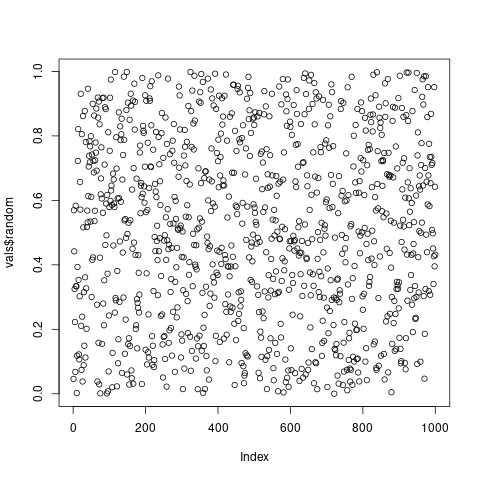
\includegraphics[width=.9\linewidth]{rand_num_plot.png}
\end{center}

\subsection{adjustl, adjustr, trim}
\label{sec:orgc47bc9a}

\begin{minted}[frame=lines,framesep=2mm,linenos=true,baselinestretch=1.2,fontsize=\footnotesize,breaklines]{fortran}
character(len=20) :: str = " gfortran "
print'(2a)', "adjustl: ", "|"//adjustl(str)                   //"|"
print'(2a)', "adjustr: ", "|"//adjustr(str)                   //"|"
print'(2a)', "trim   : ", "|"//trim(str)                      //"|"
print'(2a)', "|       |", "|"//"                             "//"|"
\end{minted}

\begin{verbatim}
adjustl: |gfortran            |
adjustr: |            gfortran|
trim   : | gfortran|
|       ||                             |
\end{verbatim}
\end{document}